%% manuscript.tex
%% IMMI Data Descriptor article (Springer Nature sn-jnl template).
%% Build with: latexmk -pdf manuscript.tex
%% Tracked changes against the submitted version: revision/make-tracked-changes.sh
\documentclass[pdflatex,sn-mathphys-num]{sn-jnl}

\usepackage{graphicx}%
\usepackage{multirow}%
\usepackage{amsmath,amssymb,amsfonts}%
\usepackage{amsthm}%
\usepackage{mathrsfs}%
\usepackage[title]{appendix}%
\usepackage{xcolor}%
\usepackage{textcomp}%
\usepackage{manyfoot}%
\usepackage{booktabs}%
\usepackage{algorithm}%
\usepackage{algorithmicx}%
\usepackage{algpseudocode}%
\usepackage{listings}%

\graphicspath{{figures/}}

\raggedbottom

\begin{document}

\title[CrabNet Hyperparameter Benchmark Dataset]{Materials Science Optimization Benchmark Dataset for High-dimensional, Multi-objective, Multi-fidelity Optimization of CrabNet Hyperparameters}

\author*[1,2]{\fnm{Sterling G.} \sur{Baird}}\email{sterling.baird@byu.edu}

\author[2]{\fnm{Xavier} \sur{Zaitzeff}}

\author[3]{\fnm{Jeet N.} \sur{Parikh}}

\author[1]{\fnm{Taylor D.} \sur{Sparks}}

\affil[1]{\orgdiv{Materials Science \& Engineering},
  \orgname{University of Utah},
  \orgaddress{\street{122 S. Central Campus Drive, \#304},
              \city{Salt Lake City}, \postcode{84112},
              \state{Utah}, \country{USA}}}

\affil[2]{\orgdiv{Mechanical Engineering},
  \orgname{Brigham Young University},
  \orgaddress{\street{701 E University Parkway, 350 EB},
              \city{Provo}, \postcode{84602},
              \state{Utah}, \country{USA}}}

\affil[3]{\orgname{Northwood High School},
  \orgaddress{\street{4515 Portola Pkwy},
              \city{Irvine}, \postcode{92620},
              \state{California}, \country{USA}}}

\abstract{Benchmarks are crucial for driving progress in scientific disciplines. To be effective, benchmarks should closely mimic real-world tasks while being computationally efficient, allowing for accessibility and repeatability. In material science and chemistry, relevant optimization tasks can be challenging due to their hierarchical, noisy, multi-fidelity, multi-objective, high-dimensional, and non-linearly correlated variables. Additionally, they may include mixed numerical and categorical variables subject to linear and non-linear constraints. This dataset is a hyperparameter optimization benchmark engineered to emulate the difficulty structure of such materials formulation problems. We generated 65,536 quasi-random combinations of 23 hyperparameters plus a training-set fraction and used them to train CrabNet, a composition-based property prediction model, on the Matbench experimental band gap task. Of 327,680 scheduled training runs, 173,219 completed (387 RTX-2080-Ti GPU days), giving 41,550 unique hyperparameter sets with 1 to 5 repeats each. The resulting regression dataset maps each hyperparameter combination to mean absolute error (MAE), root mean squared error (RMSE), computational runtime, and model size. The training-set fraction acts as a fidelity parameter: training on 30\% of the data costs about a third of the full runtime while preserving much of the ranking of hyperparameter sets. Repeated runs characterize heteroskedastic noise, and percentile ranks within each group of identical parameter sets are provided as a nonparametric description of that noise. Together with a released surrogate model, the dataset supports low-cost benchmarking of constrained, noisy, multi-objective, and multi-fidelity optimization algorithms.}

\keywords{adaptive design, Bayesian optimization, formulation optimization, hyperparameter optimization, benchmark dataset, multi-fidelity}

\maketitle

\section{Background \& Summary}\label{sec:background}

Industry-relevant optimization tasks in the physical sciences are often ``hierarchical, noisy, multi-fidelity~\cite{Existing01_Ghoreishi2019,Existing02_Kandasamy2020_Dragonfly,SabanzaGil2025_MFBO,Gantzler2023_MFBO_COF}, multi-objective~\cite{Existing03_Hanaoka2022,Existing04_Hase2018_Chimera,Ament2023_LogEI}, high-dimensional~\cite{Existing05_Baird2022_CrabNet,Existing06_Eriksson2021_SAASBO,Hvarfner2024_VanillaBO,Papenmeier2023_Bounce}, and non-linearly correlated while exhibiting mixed numerical and categorical variables subject to linear~\cite{Existing07_09_Baird2023_Compactness} and non-linear constraints.''~\cite{Existing07_09_Baird2023_Compactness,Existing08_Baird2023_HardSphere,Hickman2025_Anubis} Existing benchmark datasets~\cite{Existing10_Dunn2020_Matbench,Existing11_DeBreuck2021_MODNet,Existing12_Wang2022_ActiveLearning,Existing13_Liang2021_BO_Benchmarks,Existing14_Henderson2021,Existing15_Hase2021_Olympus,Choudhary2024_JARVIS,Hickman2025_Atlas}, while very useful, typically are single-objective, single-fidelity, low-dimensional, and ignore or simplify the influence of noise. The aim of this dataset is to better model a physical science optimization task for benchmarking needs while properly quantifying the noise distribution. This approach bridges the gap between low-cost surrogate function evaluations using benchmark datasets and costly, real-world objective function evaluations by considering a multi-objective, multi-fidelity, and high-dimensional task while accounting for heteroskedastic noise.

The scope of the dataset should be stated plainly. It is a hyperparameter optimization benchmark built on a real materials machine learning task, engineered to emulate the difficulty structure of materials formulation problems (noise that changes across the search space, a cheap fidelity parameter, mixed variable types, several competing objectives, and optional composition-like constraints). It is not a materials design benchmark in which the inputs are chemical compositions or processing conditions. General hyperparameter optimization benchmarks such as HPOBench~\cite{Eggensperger2021_HPOBench} and YAHPO Gym~\cite{Pfisterer2022_YAHPOGym} cover many machine learning models; the dataset described here adds a materials property model, measured run-to-run noise from repeated training, and constraint modes that follow the geometry of composition constraints. Growing interest in self-driving laboratories~\cite{Tom2024_SDL_Review,Abolhasani2023_SDL} and in newer composition-based models~\cite{Madani2025_TransformerGraph} increases the need for such realistic yet inexpensive test problems.

A typical materials researcher who wants to choose an optimization algorithm for an expensive campaign (for example, tuning a composition-based property model such as CrabNet, or planning a formulation study with Ax or BayBE) currently compares candidates on low-dimensional analytic test functions or on small tabular datasets, or simply uses a default. With this dataset, the same researcher can run many repeated campaigns against a surrogate of a real 24-input training process, with realistic noise, a fidelity parameter that trades accuracy for cost, and four objectives, at a cost of milliseconds per evaluation instead of GPU hours. The dataset and surrogate have already been used in this way: to compare Ax and BayBE~\cite{Fitzner2025_BayBE} strategies in public benchmarking notebooks\footnote{\url{https://github.com/AccelerationConsortium/baybe-multi-task-bo}}, through an interactive HuggingFace Space\footnote{\url{https://huggingface.co/spaces/AccelerationConsortium/crabnet-hyperparameter}}, and in an Acceleration Consortium Kaggle competition\footnote{\url{https://www.kaggle.com/datasets/acceleration-consortium/crabnet-optimization-challenge-dataset}}. We see it as the first entry in an extensible family of benchmarks: the same pipeline can be applied to other model architectures and Matbench tasks.

\section{Methods}\label{sec:methods}

\subsection{CrabNet, Matbench, and Ax}\label{sec:methods-tools}

Predicting material properties is a difficult task, and elemental composition as a predictor of material properties while the specific structure of the material is unknown is a common problem~\cite{Jha2018_ElemNet,Goodall2020_Roost,Wang2021_CrabNet}. CrabNet is a composition-based regression and classification algorithm for material properties using an attention-based neural network as a foundation~\cite{Wang2021_CrabNet}. CrabNet uses self-attention to featurize elemental composition data in the context of a chemical compound system. It has been shown to be effective in predicting material properties across several datasets and offers alternative visualizations of elemental behavior. The hyperparameters of CrabNet tune model aspects such as fitting parameters, training epochs, and network architecture, and tuning them is itself a high-dimensional optimization problem~\cite{Existing05_Baird2022_CrabNet}.

The data to train the CrabNet models was gathered from Matbench. Matbench is a collection of 13 machine learning tasks with 10 associated datasets to be used as a benchmark for novel algorithms~\cite{Existing10_Dunn2020_Matbench}. Specifically for the benchmarking task of this paper, the data used for training the CrabNet models was taken from the experimental band gap task (\texttt{matbench\_expt\_gap}, 4,604 compositions with experimentally measured band gaps~\cite{Zhuo2018_BandGapML}), which uses composition only as input and is evaluated with five-fold nested cross-validation. We chose it because composition-only inputs match CrabNet's design, the task is small enough to allow hundreds of thousands of training runs, and experimental targets make it a realistic materials task.

To ensure uniqueness and a uniform distribution across the search space, different hyperparameter combinations were generated by Ax platform's quasi-random Sobol sampling function. Ax is a machine learning package for guided experimentation~\cite{Olson2025_Ax}. It offers intuitive APIs for sampling parameter spaces and Bayesian optimization for experiment generation across high dimensional mixed datatype parameters, built on BoTorch~\cite{Balandat2020_BoTorch}. In this work, Ax was used only to generate the Sobol design; no Bayesian optimization was used to create the dataset. Sobol sequences are a deterministic low-discrepancy alternative to independent uniform sampling: each marginal is uniform, while the points fill the joint space more evenly than independent draws~\cite{Sobol1967_Sobol}.

\subsection{Search space, fidelity parameter, and constraints}\label{sec:methods-search-space}

The search space contains 20 numerical hyperparameters, 3 categorical hyperparameters, and the training-set fraction \texttt{train\_frac} (Table~\ref{tab:dictionary}). A total of 65,536 ($2^{16}$) Sobol points were generated, each was scheduled five times, and 173,219 CrabNet models were trained with the generated hyperparameter combinations with the MAE, RMSE, model size, and run time recorded as outputs. Two linear constraints were enforced when generating the design and hold for every deposited row: \texttt{betas1} $\le$ \texttt{betas2}, and \texttt{emb\_scaler} + \texttt{pos\_scaler} $\le 1$. The second constraint is a genuine three-part mixture inside CrabNet, since the weight of the logarithmic fractional encoding is set to $1 - \texttt{emb\_scaler} - \texttt{pos\_scaler}$, so the three weights always sum to one.

\texttt{train\_frac} is the only input that we frame as a fidelity parameter. Lower values train on a random subset of the training split, which lowers cost and accuracy. This mirrors common practice in large-scale machine learning, where hyperparameters are tuned on small, cheap proxy runs and then transferred to the expensive full-scale run~\cite{Yang2021_muP}, and multi-fidelity hyperparameter optimization methods that treat the training-subset size as a continuous fidelity~\cite{Klein2017_FABOLAS}. Repeats of the same hyperparameter set are not a fidelity axis; they characterize noise (Section~\ref{sec:methods-aggregation}).

While there can be other uses, this dataset is primarily intended as a multi-objective, multi-fidelity, high-dimensional benchmark dataset for formulation-based optimization scenarios by scaling each of the numerical parameters to the range of 0 to 1 and applying a deliberately synthetic constraint that the sum of the parameters must equal one. For example, discovering new materials usually means elemental composition is known and other material properties are unknown until after manufacturing. As elemental composition needs to sum to one, constraining the numerical hyperparameters mimics the form of metal alloy composition constraints found in material science type problems. CrabNet hyperparameters analogously play the role of the composition that drives unknown structural changes, and by summing to one, they ensure that trade-offs can be seen between outputs. In context of the problem, it forces optimization algorithms to balance between independent variables for better outcomes.

Concretely, the constraint is an optional benchmark mode and is not applied to the deposited data. In the \texttt{PseudoCrab} benchmark classes of the \texttt{matsci-opt-benchmarks} package, $n$ user-facing variables $x_1, \dots, x_n \in [0, 1]$ ($n = 5$, 10, or 20 depending on the difficulty tier) are mapped to $n$ of the numerical hyperparameters by min-max scaling, and a query is valid only if $\sum_{i=1}^{n} x_i \le 1$. This inequality is equivalent to a sum-to-one equality with an implicit balance component, in the same way that the balance element of an alloy is often left implicit~\cite{Existing07_09_Baird2023_Compactness}. The constraint reproduces the simplex geometry of a composition space, which is what makes composition problems hard for many optimizers; it does not reproduce the physics, chemistry, or thermodynamics of real alloys. Our working hypothesis is that if a problem looks like a formulation problem (inputs on a simplex, trade-offs between components) and responds like one, it will also optimize like one. Two limits of this hypothesis follow from the design. First, uniform sampling of the region $\sum x_i \le 1$ places most variables near their lower bounds, a region that covers a fraction $1/n!$ of the unit hypercube and therefore contains few or none of the deposited Sobol points when $n$ is large, so benchmark results in this mode rely on the surrogate away from its training data. Second, the analogy concerns the shape of the search space, not the response surface, which comes from CrabNet training rather than from materials physics.

\subsection{CrabNet training and execution environment}\label{sec:methods-execution}

For each sampled combination, CrabNet v2.0.8 (\url{https://github.com/sparks-baird/CrabNet}) was trained and evaluated on each of the five folds of \texttt{matbench\_expt\_gap}, and the reported MAE and RMSE are averages over the folds. The number of training epochs is four times \texttt{epochs\_step}, the widths of the four hidden layers of the output network are $8$, $4$, $2$, and $1$ times \texttt{out\_hidden4}, and the number of attention heads is made even with \texttt{d\_model} rounded to a multiple of it. To improve efficiency and reduce latency, hyperparameter sets (including repeats) were shuffled and divided into batches, then sent to the University of Utah's Center for High Performance Computing (CHPC) through the SLURM scheduler using Submitit for asynchronous evaluation on RTX 2080 Ti GPUs. Despite some results not being completed due to either timeout or preemption, this trade-off was deemed reasonable for the efficiency and completion gains: 52.9\% of the scheduled runs completed, and 63.4\% of the Sobol points have at least one completed run. Results were logged in JSON format to a free-tier MongoDB Atlas database through the MongoDB Data API, then aggregated and prepared as machine-learning-ready datasets via Python in Jupyter notebooks. Only runs that finished and reported scores were exported; no other filtering was applied to the deposited table.

\subsection{Aggregation and percentile ranking}\label{sec:methods-aggregation}

To realistically capture noise in the benchmark dataset and avoid bias by assuming the noise distribution, simulations were repeated for each quasi-random parameter combination. The repeats were then ranked by the ``dense'' method with \texttt{pct=True} in \texttt{pandas.core.groupby.GroupBy.rank}, and the rank was added as a feature in the surrogate model for the nondeterministic outputs of MAE, RMSE, and runtime. Model size depends only on the architecture and does not vary between repeats. The rank is a nonparametric description of where a run falls among the repeats of its set; drawing a random rank at prediction time gives a noisy surrogate output. Section~\ref{sec:tech-validation} compares this treatment with Gaussian noise models.

\section{Data Records}\label{sec:data-records}

The dataset and accompanying trained surrogates are deposited on Zenodo under a CC-BY 4.0 license with the persistent identifier \texttt{10.5281/zenodo.7694268}\footnote{\url{https://doi.org/10.5281/zenodo.7694268}}. The deposition contains the files listed in Table~\ref{tab:records}. The primary data record is \texttt{sobol\_regression.csv}; its columns are described in Table~\ref{tab:dictionary}.

\begin{table}[h]
\caption{Files in the Zenodo deposition (DOI \texttt{10.5281/zenodo.7694268}).}\label{tab:records}
\begin{tabular}{@{}p{0.32\linewidth}p{0.62\linewidth}@{}}
\toprule
\textbf{File} & \textbf{Description} \\
\midrule
\texttt{sobol\_regression.csv} & Primary data table: one row per completed CrabNet training run (173,219 rows, 35 columns; Table~\ref{tab:dictionary}). \\
\texttt{model\_metadata.json} & Metadata of the surrogate models, keyed by output (\texttt{mae}, \texttt{rmse}, \texttt{model\_size}, \texttt{runtime}). \\
\texttt{surrogate\_models.pkl} & Pickled scikit-learn random forest surrogates (scikit-learn 1.0.1) fit on the full table, one per output. \\
\texttt{cross\_validation\_models\_0.pkl} to \texttt{\_4.pkl} & Surrogates fit on five cross-validation splits of the table, for held-out evaluation of the surrogate. \\
\bottomrule
\end{tabular}
\end{table}

\begin{table}[h]
\caption{Data dictionary for \texttt{sobol\_regression.csv}. Integer hyperparameters are marked (int). Bounds are those of the Sobol design.}\label{tab:dictionary}
\footnotesize
\begin{tabular}{@{}p{0.24\linewidth}p{0.22\linewidth}p{0.48\linewidth}@{}}
\toprule
\textbf{Column} & \textbf{Type and range} & \textbf{Description} \\
\midrule
\texttt{\_id}, \texttt{session\_id}, \texttt{timestamp} & string, string, float & MongoDB record identifier, batch session identifier, Unix time of the record (s) \\
\texttt{N} & int, 1 to 10 & number of attention layers \\
\texttt{d\_model} & int, 100 to 1024 & model (embedding) dimension \\
\texttt{dim\_feedforward} & int, 1024 to 4096 & width of the feed-forward sublayers \\
\texttt{heads} & int, 1 to 10 & number of attention heads \\
\texttt{dropout} & float, 0 to 1 & dropout probability \\
\texttt{emb\_scaler}, \texttt{pos\_scaler} & float, 0 to 1 each, sum $\le 1$ & weights of the element embedding and of the fractional encoding (the log fractional encoding receives the remainder) \\
\texttt{pe\_resolution}, \texttt{ple\_resolution} & int, 2500 to 10000 & resolution of the fractional and log fractional encodings \\
\texttt{fudge} & float, 0 to 0.1 & random perturbation of element fractions during training \\
\texttt{out\_hidden4} & int, 32 to 512 & width of the last hidden layer of the output network \\
\texttt{bias} & boolean & CrabNet \texttt{bias} flag \\
\texttt{epochs\_step} & int, 5 to 20 & training epochs divided by four \\
\texttt{batch\_size} & int, 32 to 256 & batch size \\
\texttt{lr} & float, $10^{-4}$ to $6\times10^{-3}$ & learning rate \\
\texttt{weight\_decay} & float, 0 to 1 & weight decay \\
\texttt{eps} & float, $10^{-7}$ to $10^{-4}$ & optimizer epsilon \\
\texttt{betas1}, \texttt{betas2} & float, 0.5 to 0.9999, \texttt{betas1} $\le$ \texttt{betas2} & optimizer beta coefficients \\
\texttt{alpha}, \texttt{k} & float 0 to 1, int 2 to 10 & Lookahead optimizer step size and synchronization period \\
\texttt{criterion} & RobustL1, RobustL2 & loss function \\
\texttt{elem\_prop} & mat2vec, magpie, onehot & element featurization \\
\texttt{train\_frac} & float, 0.01 to 1 & fraction of each training split used (fidelity parameter); 16 rows from two small test sessions use 0.003 \\
\texttt{hardware} & string & GPU model (\texttt{2080ti} for all rows) \\
\texttt{mae}, \texttt{rmse} & float (eV) & MAE and RMSE averaged over the five Matbench folds \\
\texttt{runtime} & float (s) & wall-clock time of the run (all five folds) \\
\texttt{model\_size} & int & number of trainable parameters \\
\texttt{mae\_rank}, \texttt{rmse\_rank}, \texttt{runtime\_rank} & float, 0 to 1 & dense percentile rank of the output within the repeats of the same hyperparameter set \\
\bottomrule
\end{tabular}
\end{table}

The record is designed to support the FAIR principles~\cite{Wilkinson2016_FAIR}. It is findable through a persistent DOI with descriptive metadata, accessible through open download without authentication, interoperable through plain CSV and JSON files with the schema in Table~\ref{tab:dictionary}, and reusable through an open license, the provenance described in Section~\ref{sec:methods}, and the versioned code in Section~\ref{sec:code}. The pickled surrogates require the scikit-learn version stated above.

\section{Technical Validation}\label{sec:tech-validation}

Figure~\ref{fig:histograms} summarizes the deposited table. Among the 41,550 unique hyperparameter sets, the number of completed repeats ranges from 1 to 5 with a mean of 4.17 (Figure~\ref{fig:histograms}a). The value of approximately 2.6 given in the submitted version was the number of completed runs per scheduled Sobol point (173,219 / 65,536), which includes the 36.6\% of points with no completed run. MAE ranges from 0.169 to 1.214~eV and RMSE from 0.440 to 1.703~eV, both less than one order of magnitude. Runtime spans about four orders of magnitude (2.8~s to $3.4\times10^{4}$~s, with 31 runs longer than one hour), and model size spans about two (from $2.0\times10^{6}$ to $1.2\times10^{8}$ trainable parameters).

\begin{figure}[h]
\centering
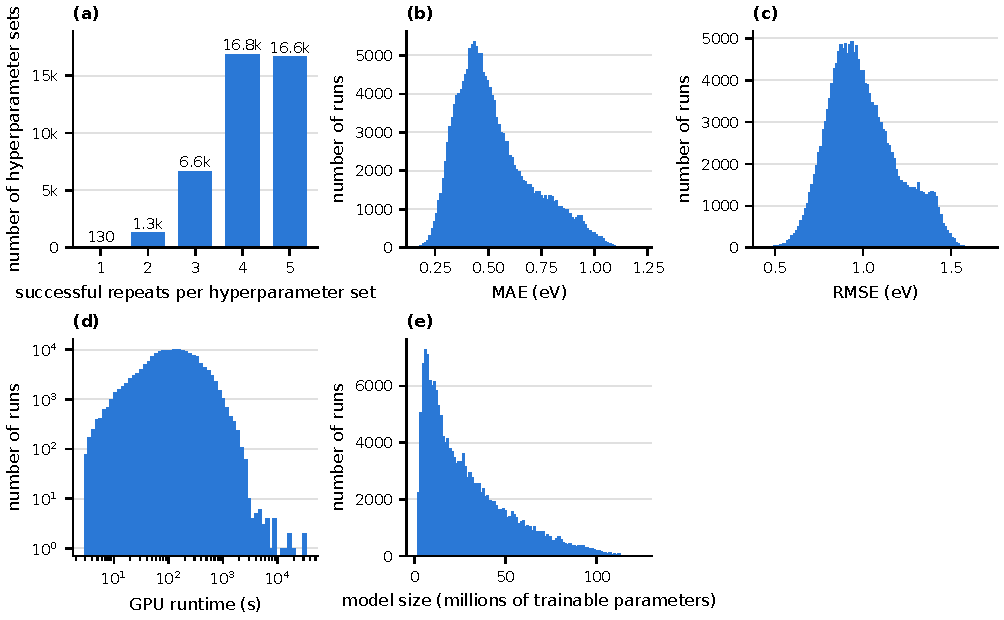
\includegraphics[width=\linewidth]{histograms_panel.pdf}
\caption{Distributions in the deposited table. (a) Number of completed repeats per unique hyperparameter set (41,550 sets, mean 4.17). (b) MAE, (c) RMSE, (d) GPU runtime on one RTX 2080 Ti (both axes logarithmic, since runtime spans about four orders of magnitude), and (e) model size in millions of trainable parameters, over all 173,219 completed runs of CrabNet on the Matbench experimental band gap task.}
\label{fig:histograms}
\end{figure}

The four outputs show genuine trade-offs (Figure~\ref{fig:pareto}). MAE and RMSE are strongly correlated (Spearman $\rho = 0.97$ on repeat-averaged data), so they act largely as one accuracy objective. Accuracy trades off against cost: MAE and RMSE are negatively correlated with runtime ($\rho = -0.57$ and $-0.61$), giving Pareto fronts with 65 and 52 non-dominated sets. Model size is nearly independent of accuracy ($|\rho| \le 0.07$) and weakly correlated with runtime ($\rho = 0.37$). The released surrogate, evaluated at the median noise rank, reproduces every pairwise correlation to within 0.02, which supports its use in place of the raw data.

\begin{figure}[h]
\centering
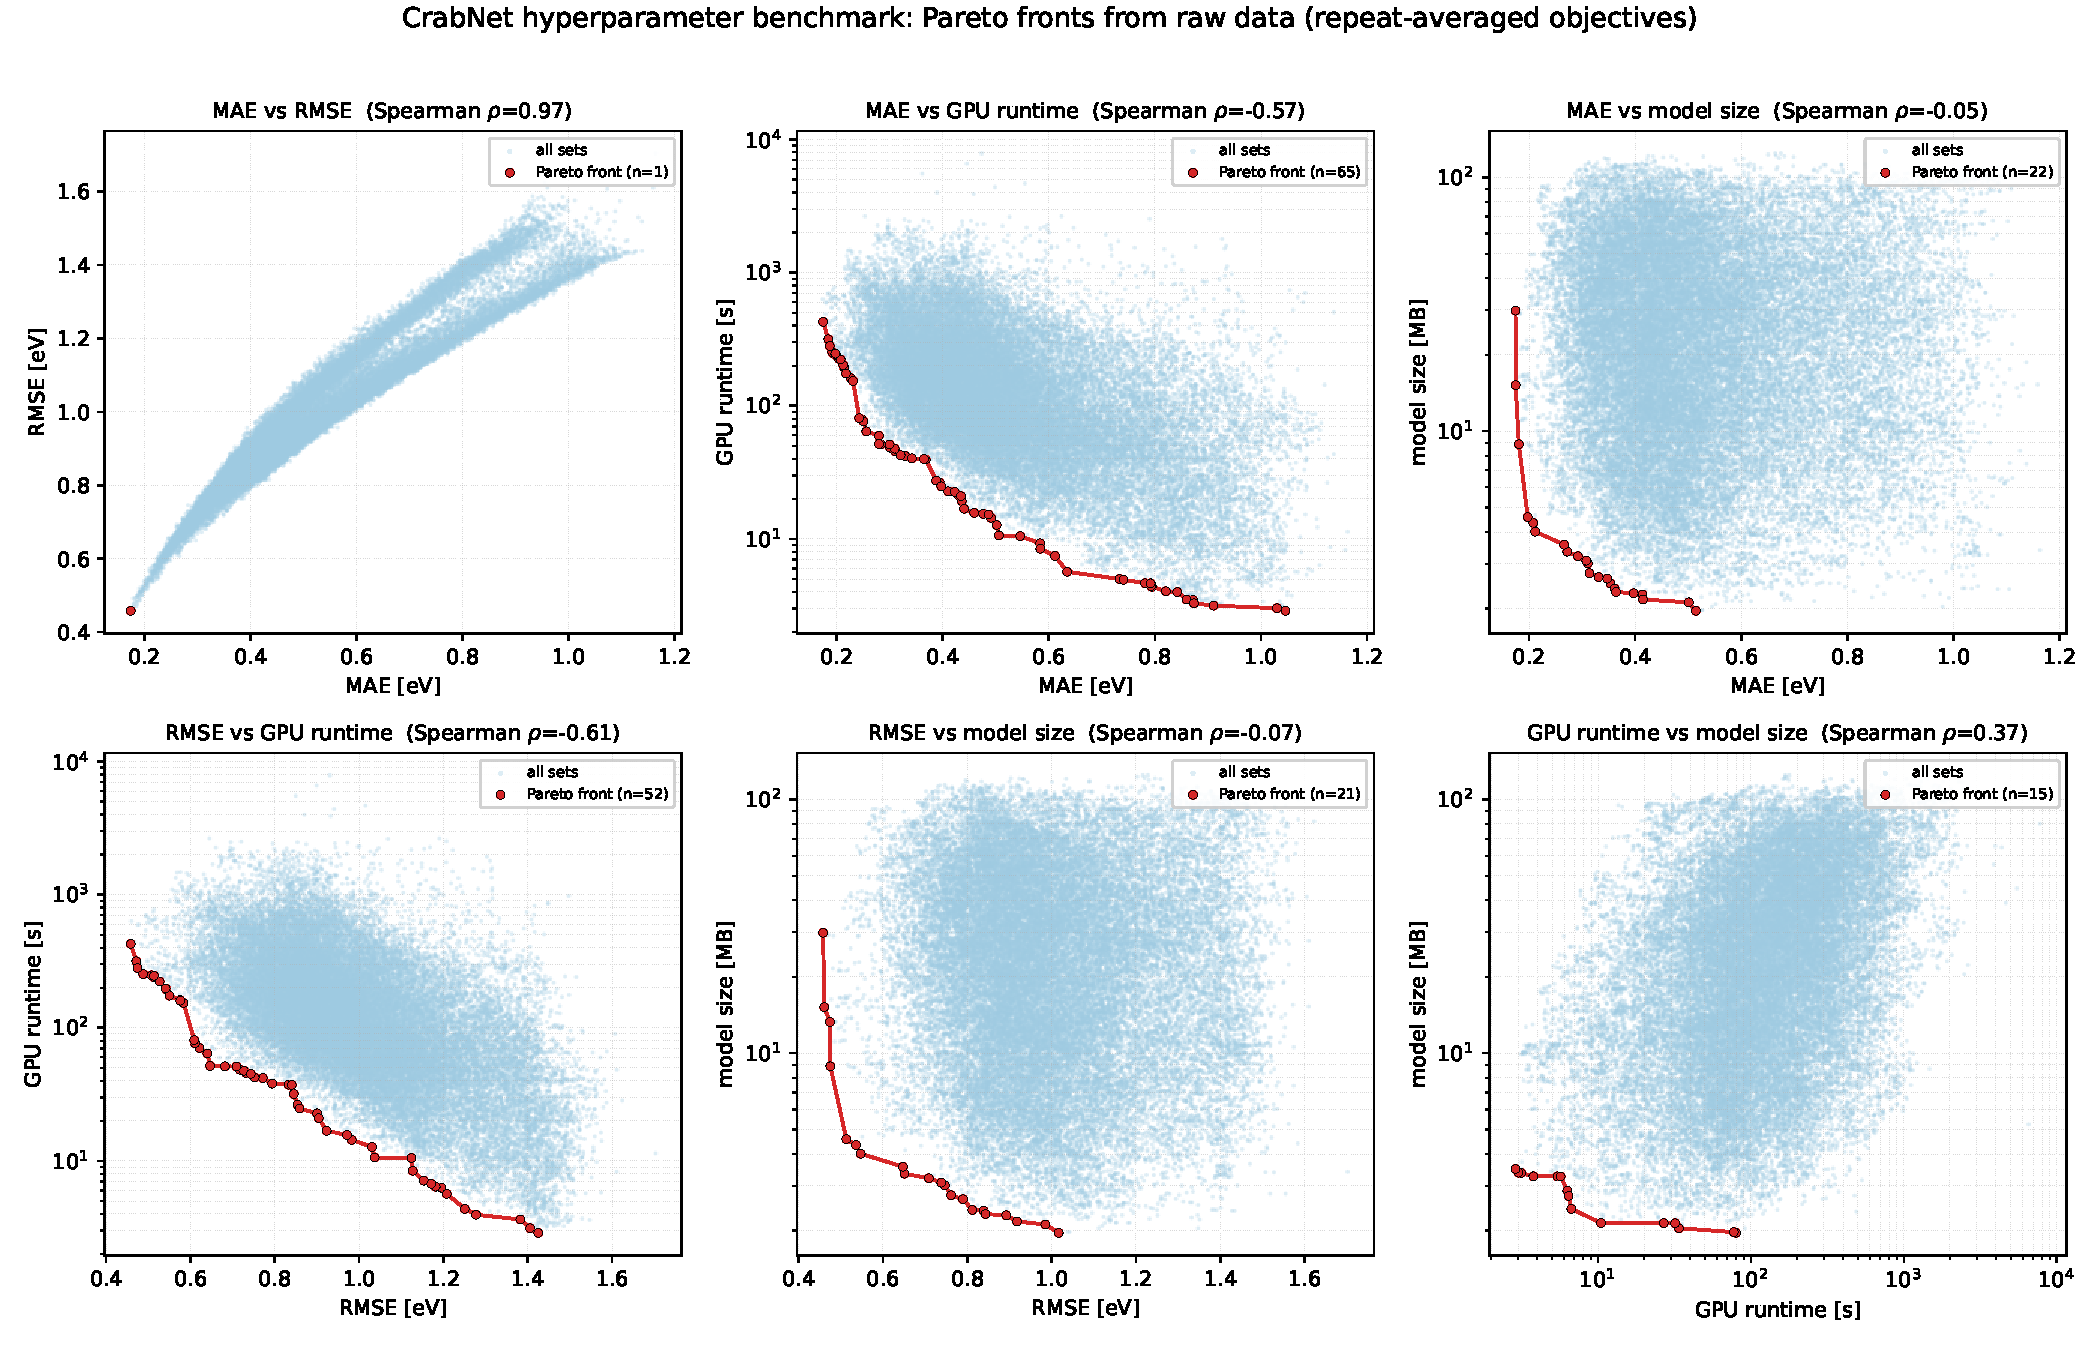
\includegraphics[width=\linewidth]{pareto_rawdata.pdf}\\[2pt]
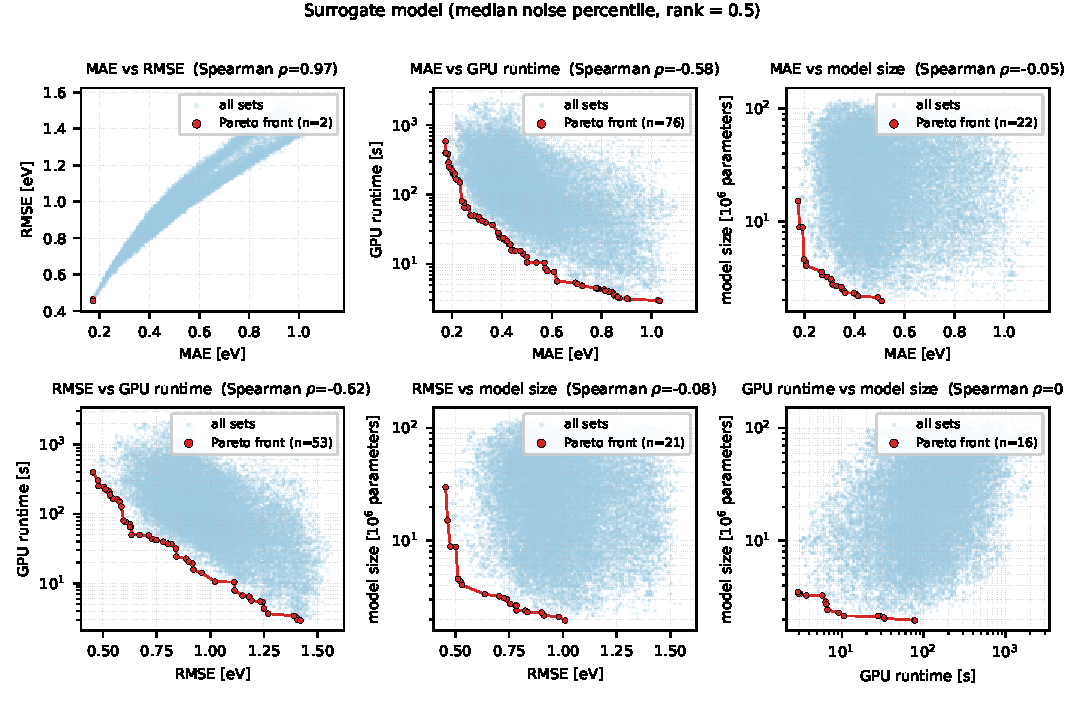
\includegraphics[width=\linewidth]{pareto_surrogate.pdf}
\caption{Pairwise Pareto fronts (red) of the four minimized outputs. Top six panels: raw data, averaged over the repeats of each of the 41,550 hyperparameter sets. Bottom six panels: the released surrogate evaluated at the same hyperparameter sets with the noise rank fixed at the median (0.5). Panel titles give the Spearman rank correlation.}
\label{fig:pareto}
\end{figure}

The fidelity parameter behaves as intended (Figure~\ref{fig:fidelity}). For 5,000 deposited hyperparameter sets, we used the surrogate to predict MAE and runtime at several values of \texttt{train\_frac}. Rankings of the sets at reduced fidelity agree with those at full fidelity (Spearman $\rho = 0.77$ at \texttt{train\_frac} = 0.1, 0.84 at 0.3, and 0.93 at 0.5), while the median runtime falls to 14\%, 33\%, and 56\% of the full-fidelity value. About half of the best 10\% of sets at \texttt{train\_frac} = 0.3 are also in the best 10\% at full fidelity. Low-fidelity evaluations are therefore informative but imperfect, which is the setting multi-fidelity optimizers are designed for.

\begin{figure}[h]
\centering
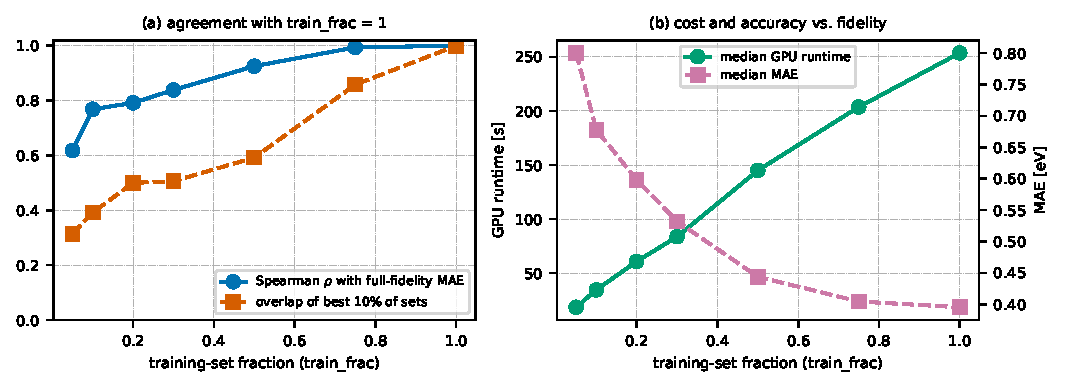
\includegraphics[width=\linewidth]{fidelity_surrogate.pdf}
\caption{The training-set fraction as a fidelity parameter, from surrogate predictions (median noise rank) for 5,000 deposited hyperparameter sets. (a) Spearman correlation between MAE at a given \texttt{train\_frac} and MAE at \texttt{train\_frac} = 1, and overlap of the best 10\% of sets. (b) Median GPU runtime and median MAE as a function of \texttt{train\_frac}.}
\label{fig:fidelity}
\end{figure}

Repeated runs show that the noise is heteroskedastic. Within a hyperparameter set, the standard deviation of MAE varies 14-fold between the 5th and 95th percentiles of sets (0.003 to 0.047~eV) and that of runtime 190-fold (0.4 to 68~s), and both increase with the set mean (Spearman $\rho = 0.33$ and $0.68$). Standardized residuals are nearly symmetric for MAE (skewness 0.07) but skewed for runtime (0.68). To test the percentile-rank treatment, we split the sets with at least three repeats into 80\% training and 20\% held-out sets (8,025 held-out sets, 34,288 runs) and fit the same gradient-boosting learner to three noise models: a rank-conditioned model (the approach used for the released surrogate), a constant-variance Gaussian, and a Gaussian whose standard deviation is predicted from the hyperparameters (Figure~\ref{fig:noise}). By the continuous ranked probability score (CRPS)~\cite{Gneiting2007_ScoringRules}, the rank-conditioned model was best for runtime, whose noise is skewed (22.8~s, against 25.6~s for the heteroskedastic Gaussian and 34.0~s for the constant-variance Gaussian), while the heteroskedastic Gaussian was best for MAE (0.0166~eV, against 0.0171~eV and 0.0181~eV for the constant-variance and rank-conditioned models). The rank-conditioned intervals were too narrow for both outputs (their central 80\% interval contained 37\% of held-out MAE values and 23\% of runtimes), because the ranks describe run-to-run spread but not the surrogate's own error at unseen hyperparameters. The percentile ranks are therefore a useful nonparametric description of the measured repeats, most valuable for skewed outputs such as runtime, and users who need calibrated intervals should add an estimate of surrogate error.

\begin{figure}[h]
\centering
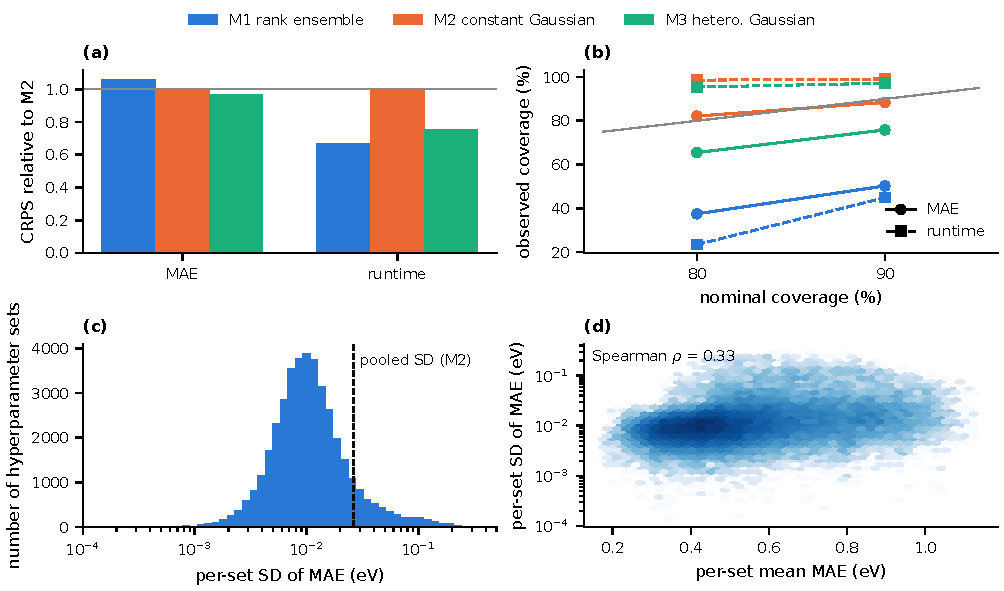
\includegraphics[width=\linewidth]{noise_ablation.pdf}
\caption{Noise models compared on held-out hyperparameter sets (80/20 split by unique set; gradient-boosted tree models). M1: rank-conditioned model as in the released surrogate, with a predictive ensemble from 21 evenly spaced ranks. M2: Gaussian with a constant standard deviation equal to the pooled within-set value. M3: Gaussian with a per-set standard deviation predicted from the hyperparameters. (a) Mean CRPS relative to M2 (lower is better). (b) Observed coverage of central 80\% and 90\% intervals against nominal coverage. (c) Per-set standard deviation of MAE across repeats; the dashed line is the pooled value used by M2. (d) Per-set standard deviation of MAE against per-set mean MAE.}
\label{fig:noise}
\end{figure}

\IfFileExists{figures/optimizer_benchmark.pdf}{%
To show how the benchmark separates optimization strategies, we ran repeated single-objective campaigns (minimize MAE at \texttt{train\_frac} = 1, both native constraints enforced, noisy observations drawn with a random noise rank, 50 evaluations each) with random search, grid search, Sobol and Latin hypercube~\cite{McKay1979_LHS} designs, a genetic algorithm~\cite{Blank2020_Pymoo}, Ax with its default Bayesian optimization strategy, Ax with SAASBO~\cite{Existing06_Eriksson2021_SAASBO}, and BoFire~\cite{Durholt2024_BoFire} (Figure~\ref{fig:optimizers}). The number of repeated campaigns per method is given in the figure.

\begin{figure}[h]
\centering
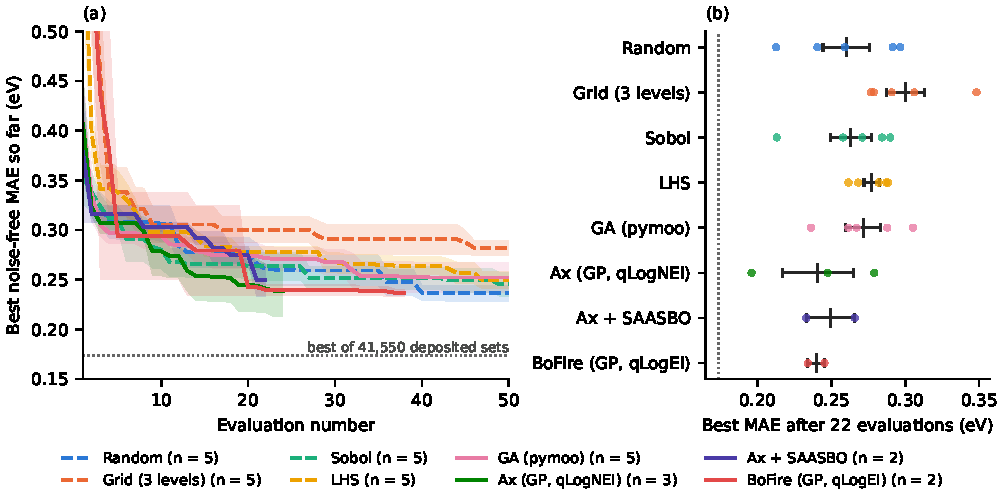
\includegraphics[width=\linewidth]{optimizer_benchmark.pdf}
\caption{Best noise-free MAE found so far (surrogate at median noise rank) as a function of the number of evaluations, averaged over repeated campaigns (shaded band: standard error) for each optimization strategy.}
\label{fig:optimizers}
\end{figure}
}{}

\section{Usage Notes}\label{sec:usage}

The primary table \texttt{sobol\_regression.csv} can be loaded directly with \texttt{pandas.read\_csv}. To use the dataset as a benchmark, we recommend the trained surrogate (\texttt{surrogate\_models.pkl}), which maps any in-bounds hyperparameter vector and a noise rank to predicted MAE, RMSE, runtime, and model size. Drawing the rank uniformly at random gives noisy evaluations; fixing it at 0.5 gives a noise-free reference value for scoring. Queries should respect the two native constraints, and \texttt{train\_frac} should be treated as the fidelity parameter, with runtime as its cost. The optional sum constraint is available through the \texttt{PseudoCrab} classes of the \texttt{matsci-opt-benchmarks} package. The HuggingFace Space and the BayBE and Ax notebooks listed in Section~\ref{sec:background} are working templates for new benchmarking studies; they are not part of the formal data record.

\section{Code availability}\label{sec:code}

All code used to generate, aggregate, and analyze the dataset is openly available in the \texttt{matsci-opt-benchmarks} repository (\url{https://github.com/sparks-baird/matsci-opt-benchmarks}), including the orchestration script \texttt{scripts/crabnet\_hyperparameter/crabnet\_hyperparameter\_submitit.py}, the data preparation and surrogate fitting notebooks in \texttt{notebooks/crabnet\_hyperparameter}, and the scripts that produce the figures in this article. The source state used to generate the dataset is archived on Zenodo as release v0.2.1 (\url{https://doi.org/10.5281/zenodo.7694289}). The CrabNet implementation used for training is at \url{https://github.com/sparks-baird/CrabNet} (version 2.0.8).

\section*{CRediT author statement}

\textbf{Sterling G.~Baird}: Project administration, Conceptualization, Methodology, Software, Validation, Formal analysis, Investigation, Data Curation, Writing - Original Draft, Writing - Review \& Editing, Visualization. \textbf{Xavier Zaitzeff}: Writing - Original Draft, Writing - Review \& Editing. \textbf{Jeet N.~Parikh}: Methodology, Software, Formal Analysis, Data Curation, Writing - Original Draft, Writing - Review \& Editing. \textbf{Taylor D.~Sparks}: Supervision, Funding acquisition.

\section*{Acknowledgments}

Funding: This work was supported by the National Science Foundation Division of Materials Research [Grant number DMR-1651668].

We thank Trupti Mohanty for discussion related to the future use-case of this dataset as an optimization benchmark. We acknowledge the University of Utah's Center for High Performance Computing (CHPC) for providing computational resources. The code and manuscript associated with a benchmark dataset for particle packing simulations~\cite{Existing08_Baird2023_HardSphere} served as a starting point for the code and manuscript for this work, for which there is shared language and document structure. We acknowledge OpenAI for providing free usage of their research tool, ChatGPT, which was used during the review and editing process, and Anthropic's Claude, which was used to prepare revision analyses and edits.

\section*{Declaration of interests}

The authors declare that they have no known competing financial interests or personal relationships that could have appeared to influence the work reported in this paper.

\bibliography{references}

\end{document}
